\documentclass{article}
\usepackage[utf8]{inputenc}
\usepackage{multicol}
\usepackage{listings}
\usepackage{verbatim}
\usepackage{color}
\usepackage{geometry}
\usepackage{float}
\usepackage{amsmath}
\usepackage{caption}
\usepackage{pdflscape}
\usepackage{hyperref}
\setlength{\belowcaptionskip}{-10pt}
\setlength{\abovecaptionskip}{-30pt}
\floatstyle{boxed} 
\restylefloat{figure}
\usepackage{graphicx}
\definecolor{codegreen}{rgb}{0,0.6,0}
\definecolor{codegray}{rgb}{0.5,0.5,0.5}
\definecolor{codepurple}{rgb}{0.58,0,0.82}
\definecolor{backcolour}{rgb}{0.95,0.95,0.92}
\lstdefinestyle{mystyle}{
	backgroundcolor=\color{backcolour},   
	commentstyle=\color{codegreen},
	keywordstyle=\color{blue},
	numberstyle=\tiny\color{codegray},
	stringstyle=\color{codepurple},
	basicstyle=\footnotesize,
	breakatwhitespace=false,         
	breaklines=true,                 
	captionpos=b,                    
	keepspaces=true,                 
	numbers=left,                    
	numbersep=5pt,                  
	showspaces=false,                
	showstringspaces=false,
	showtabs=false,                  
	tabsize=2
}
\lstset{style=mystyle}
\title{Data Mining\\
		Home work 09\\Machine Learning Part:2 }
\author{Aqeel Labash\\ \textbf{Lecturer:} Jaak Vilo}
\date{06 April 2016}
\geometry{
	a4paper,
	total={170mm,257mm},	
	left=10mm,
	top=5mm,
}
\begin{document}
	\maketitle
\section*{First Question}
The article focus on classification. And here is the list 
\begin{itemize}
	\item No matter what algorithm you pick it's consist from three parts : Representation, Evaluation, Optimization.
	\item \textbf{Representation:} The feature we want to use in away computer can handle.
	\item \textbf{Evaluation or objective or scoring function:} used to distinguish between good and bad classifiers.
	\item \textbf{Optimization :} a method that search for best scoring classifiers.
	\item Generalization is what we want. "if there are 100,000 words in the dictionary, the spam filter described above has 2100,000 possible different inputs."
	\item Always test your module on data different than the train data.
	\item data by itself is not enough for generalization knowledge is also required to know which module to apply."A corollary of this is that one of the key criteria for choosing a representation is which kinds of knowledge are easily expressed in it. For example, if we have a lot of knowledge about what makes examples similar in our domain, instance-based methods may be a good choice. If we have knowledge about probabilistic dependencies, graphical models are a good fit.And if we have knowledge about what kinds of preconditions are required by each class, “IF . . . THEN . . .” rules may be the best option."
	\item \textbf{Over fitting} could be decomposed to Bias and Variance."Bias is a learner’s tendency to consistently learn the same wrong thing.Variance is the tendency to learn random things irrespective of the real signal." 
	\item Some ways to fight over fitting is: regularization term, cross validation, statistical significance.
	\item In most cases over fitting doesn't happen because of noise.
	\item intuitions used for low dimension usually don't  work with high dimension problems."our intuitions, which come from a three-dimensional world, often do not apply in high-dimensional ones."
	\item Numbers in theory might not be applicable and not always correct."consider the space of Boolean functions of d Boolean variables. If there are e possible different examples, there are \(2^e\) possible different functions, so since there are \(2^d\) possible examples,the total number of functions is \(2^{2^d}\).And even for hypothesis spaces that are “merely” exponential, the bound is still very loose, because the union bound is very pessimistic. For example, if there are 100 Boolean features and the hypothesis space is decision trees with up to 10 levels, to guarantee \(\delta = \epsilon = 1\%\) in the bound above we need half a million examples. But in practice a small fraction of this suffices for accurate learning."
	\item \textbf{Good Features:}are those which independent from each other and highly correlated with the class.
	\item Awesome feature is not necessarily provided by the data we might have to build it."Often, the raw data is not in a form that is amenable to learning, but you can construct features from it that are."
	\item The algorithm with more data wins."As a rule of thumb, a dumb algorithm with lots and lots of data beats a clever one with modest amounts of it. (After all, machine learning is all about letting data do the heavy lifting.)"
	\item The more data we have, the more complex the classifier.
	\item "Variable size learners can in principle learn any function given sufficient data, but in	practice they may not, because of limitations of the algorithm (for example,greedy search falls into local optima) or computational cost."
	\item Ensemble learning give better results usually.
	\item if the classifier is simpler doesn't mean it's more accurate.
	\item being able to represent the data doesn't mean that module can learn it."For example, standard decision tree learners cannot learn trees with more leaves than there are training examples."
	\item correlation doesn't mean one cause another.it's just an observation on the data that might have cause relation.
\end{itemize}
\section*{Second Question}
For this task I used the following Code : 
\begin{lstlisting}[language=Python]

import matplotlib.pyplot as plt


# In[2]:

original = {}
TotalPositive = 0
TotalNegative = 0
with open('data.class','r') as f:
f = f.readlines()
for line in f:
line = line.split()
if line[1]=='T':
original[line[0]]=True 
TotalPositive+=1
else:
original[line[0]]=False 
TotalNegative+=1
roc1=[]
with open('roc1.txt','r') as f:
f = f.readlines()
for line in f:
roc1.append(line.strip())
roc2=[]
with open('roc2.txt','r') as f:
f = f.readlines()
for line in f:
roc2.append(line.strip())
roc3=[]
with open('roc3.txt','r') as f:
f = f.readlines()
for line in f:
roc3.append(line.strip())
roc4=[]
with open('roc4.txt','r') as f:
f = f.readlines()
for line in f:
roc4.append(line.strip())
rocperfect = []
for x in original.keys():
if original[x]:
rocperfect = [x]+rocperfect
else:
rocperfect.append(x)


# In[3]:

def GetTPFP(k,dataset):
TP=0
FP=0
TN=0
FN=0
for i in range (3000):
#Identified True
if i<k:
TP+=original[dataset[i]]
else:
TN+=original[dataset[i]]
#(TP,FP,TN,FN)
#(F11,F01,F10,F00)
#return (TP,TotalPositive-TP,TN,TotalNegative-TN)
return (float (TP)/float(TotalPositive),float(k-TP)/float(TotalNegative))



# In[4]:

roc1cm=[]
roc2cm=[]
roc3cm=[]
roc4cm=[]
rocperfectcm=[]
print 'processing roc1'
for i in range (3000):
roc1cm.append(GetTPFP(i,roc1))
print 'processing roc2'
for i in range (3000):
roc2cm.append(GetTPFP(i,roc2))
print 'processing roc3'
for i in range (3000):
roc3cm.append(GetTPFP(i,roc3))
print 'processing roc4'
for i in range (3000):
roc4cm.append(GetTPFP(i,roc4))
print 'processing rocperfect'
for i in range (3000):
rocperfectcm.append(GetTPFP(i,rocperfect))
print 'Finished'


# In[5]:

plt.figure('roc1.jpg')
plt.plot([x[1] for x in roc1cm],[x[0] for x in roc1cm], 'ro')
plt.ylabel('TPR')
plt.xlabel('FPR')
plt.title('Roc1')
#plt.show()
plt.savefig('roc1.jpg')


# In[6]:

plt.figure('roc2.jpg')
plt.plot([x[1] for x in roc2cm],[x[0] for x in roc2cm], 'ro')
plt.ylabel('TPR')
plt.xlabel('FPR')
plt.title('Roc2')
#plt.show()
plt.savefig('roc2.jpg')


# In[7]:

plt.figure('roc3.jpg')
plt.plot([x[1] for x in roc3cm],[x[0] for x in roc3cm], 'ro')
plt.ylabel('TPR')
plt.xlabel('FPR')
plt.title('Roc3')
#plt.show()
plt.savefig('roc3.jpg')


# In[8]:

plt.figure('roc4.jpg')
plt.plot([x[1] for x in roc4cm],[x[0] for x in roc4cm], 'ro')
plt.ylabel('TPR')
plt.xlabel('FPR')
plt.title('Roc4')
#plt.show()
plt.savefig('roc4.jpg')


# In[9]:

plt.figure('rocperfect.jpg')
plt.plot([x[1] for x in rocperfectcm],[x[0] for x in rocperfectcm], 'ro')
plt.ylabel('TPR')
plt.xlabel('FPR')
plt.title('Rocperfect')
#plt.show()
plt.savefig('rocperfect.jpg')


# In[10]:

AUCROC1=0
AUCROC2=0
AUCROC3=0
AUCROC4=0
AUCROCPERFECT=0

for i in range(1,3000):
AUCROC1+= (roc1cm[i][1]-roc1cm[i-1][1])*roc1cm[i][0]
AUCROC2+= (roc2cm[i][1]-roc2cm[i-1][1])*roc2cm[i][0]
AUCROC3+= (roc3cm[i][1]-roc3cm[i-1][1])*roc3cm[i][0]
AUCROC4+= (roc4cm[i][1]-roc4cm[i-1][1])*roc4cm[i][0]
AUCROCPERFECT+= (rocperfectcm[i][1]-rocperfectcm[i-1][1])*rocperfectcm[i][0]

print AUCROC1,AUCROC2,AUCROC3,AUCROC4,AUCROCPERFECT
\end{lstlisting}
What  I did in the previous is simply calculated TP and from it I calculated TPR \& FPR.
\[TPR = \frac{TP}{TP+FN}\]
\[FPR = \frac{FP}{FP+TN} = 1 - specificity \]
 the confusion matrix and from it I calculated TPR,FPR then draw them.And here is the figures :\\
\begin{figure}[H]
	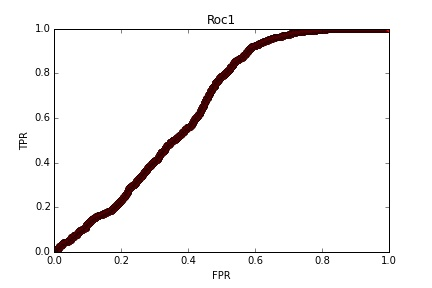
\includegraphics[scale=0.58]{roc1.jpg}
	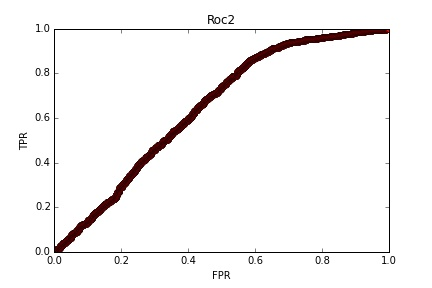
\includegraphics[scale=0.58]{roc2.jpg}\\
	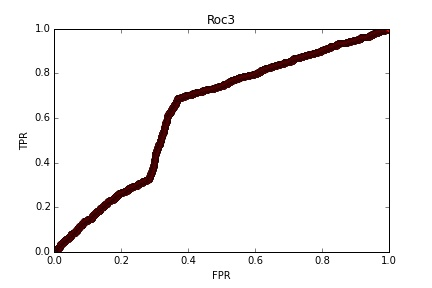
\includegraphics[scale=0.58]{roc3.jpg}		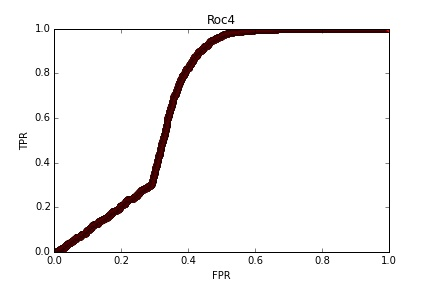
\includegraphics[scale=0.58]{roc4.jpg}
	\begin{center}
	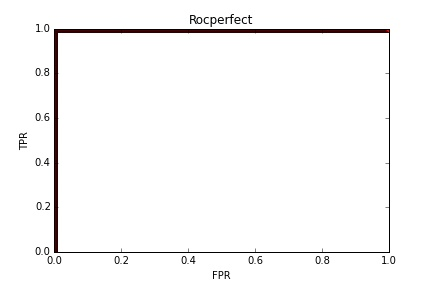
\includegraphics[scale=0.58]{rocperfect.jpg}
	\end{center}

	\caption{ROC for all the predictions.}
\end{figure}
We can notice from the previous figures that Roc4 give a good prediction for TP and minimum FP compared to others.\\
\textbf{Note:}I added a plot for the perfect file how the perfect classifier would look like.
The following code calculate approximation of the area under curve.We calculate the sum of all rectangles (point by point) and so on.
\begin{lstlisting}[language=R]
AUCROC1=0
AUCROC2=0
AUCROC3=0
AUCROC4=0

for i in range(1,3000):
AUCROC1+= (roc1cm[i][1]-roc1cm[i-1][1])*roc1cm[i][0]
AUCROC2+= (roc2cm[i][1]-roc2cm[i-1][1])*roc2cm[i][0]
AUCROC3+= (roc3cm[i][1]-roc3cm[i-1][1])*roc3cm[i][0]
AUCROC4+= (roc4cm[i][1]-roc4cm[i-1][1])*roc4cm[i][0]
print AUCROC1,AUCROC2,AUCROC3,AUCROC4
\end{lstlisting}
The previous code give the following result :
\[AUC1=0.650940277346,AUC2= 0.647270924831,AUC3= 0.629960231006,AUC4= 0.696844993141\]
\section*{Third Question}
To charactraize the previous plots.I would explain what is happening.When we start we predict 0 or 1 positive so TP+FP =1 at best cases, while k is growing TP+FP is growing as well.At the end we predict all the data as True.In that point we have \(TPR =1 , FPR =1 \).\\
The previous figures 
For this task I used the hint for this question so I subtracted FPR from TPR and then tried to find the max value. I used the following code :
\begin{lstlisting}[language=Python]
def FindK(dataset):
k=0
lst=[]
for i in range (3000):
lst.append({'x':i,'y':dataset[i][0]-dataset[i][1]})

lst.sort(key=lambda x: x['y'], reverse=True)
return lst[0]['x']
print FindK(roc1cm),FindK(roc2cm),FindK(roc3cm),FindK(roc4cm)
roc1best = FindK(roc1cm)
roc2best = FindK(roc2cm)
roc3best = FindK(roc3cm)
roc4best = FindK(roc4cm)
rocperfectbest= FindK(rocperfectcm)
print roc1best,roc2best,roc3best,roc4best,rocperfectbest
\end{lstlisting}
the previous code output the following data :
\[roc1best:2179,roc2best:2089,roc3best:1500,roc4best:1996,rocperfectbest:1215\]
To get better view I drawn the data and pointed out those points using the following code:
\begin{lstlisting}[language=Python]
plt.figure('roc1_best.jpg')
plt.plot([x[1] for x in roc1cm],[x[0] for x in roc1cm], 'ro')
plt.ylabel('TPR')
plt.xlabel('FPR')
plt.title('Roc1 Best Point')
plt.axvline(x=roc1cm[roc1best][1])
plt.axhline(y=roc1cm[roc1best][0])
#plt.show()
plt.savefig('roc1_best.jpg')


# In[24]:

plt.figure('roc2_best.jpg')
plt.plot([x[1] for x in roc2cm],[x[0] for x in roc2cm], 'ro')
plt.ylabel('TPR')
plt.xlabel('FPR')
plt.title('Roc2 Best Point')
plt.axvline(x=roc2cm[roc2best][1])
plt.axhline(y=roc2cm[roc2best][0])
#plt.show()
plt.savefig('roc2_best.jpg')


# In[25]:

plt.figure('roc3_best.jpg')
plt.plot([x[1] for x in roc3cm],[x[0] for x in roc3cm], 'ro')
plt.ylabel('TPR')
plt.xlabel('FPR')
plt.title('Roc3 Best Point')
plt.axvline(x=roc3cm[roc3best][1])
plt.axhline(y=roc3cm[roc3best][0])
#plt.show()
plt.savefig('roc3_best.jpg')


# In[27]:

plt.figure('roc4_best.jpg')
plt.plot([x[1] for x in roc4cm],[x[0] for x in roc4cm], 'ro')
plt.ylabel('TPR')
plt.xlabel('FPR')
plt.title('Roc4 Best Point')
plt.axvline(x=roc4cm[roc4best][1])
plt.axhline(y=roc4cm[roc4best][0])
#plt.show()
plt.savefig('roc4_best.jpg')


# In[28]:

plt.figure('rocperfect_best.jpg')
plt.plot([x[1] for x in rocperfectcm],[x[0] for x in rocperfectcm], 'ro')
plt.ylabel('TPR')
plt.xlabel('FPR')
plt.title('Rocperfect Best Point')
plt.axvline(x=rocperfectcm[rocperfectbest][1])
plt.axhline(y=rocperfectcm[rocperfectbest][0])
#plt.show()
plt.savefig('rocperfect_best.jpg')
\end{lstlisting}
The previous code output the following figures : 
\begin{figure}[H]
	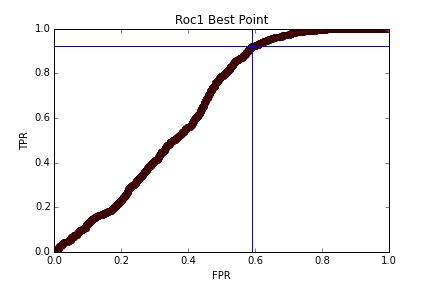
\includegraphics[scale=0.58]{roc1_best.jpg}
	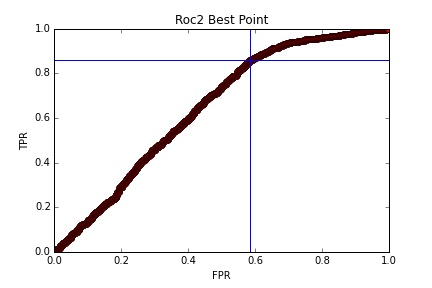
\includegraphics[scale=0.58]{roc2_best.jpg}\\
	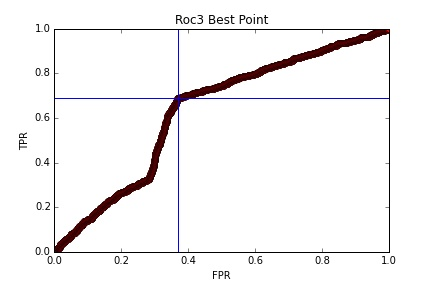
\includegraphics[scale=0.58]{roc3_best.jpg}		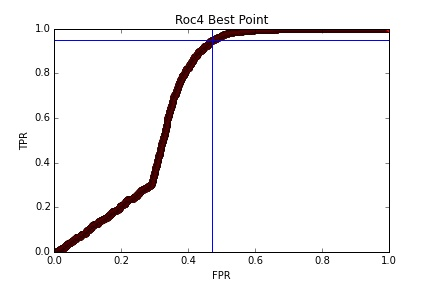
\includegraphics[scale=0.58]{roc4_best.jpg}
	\begin{center}
		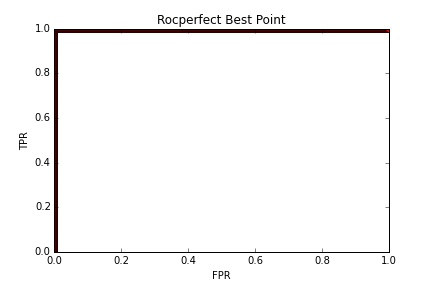
\includegraphics[scale=0.58]{rocperfect_best.jpg}
	\end{center}
	
	\caption{ROC for all the predictions pointing the best split point.}
\end{figure}
From the previous figure we can see that at the "Rocperfect" we can't see the blue lines that's because they overlap with the data itself.\\
\textbf{Note: }second and third question code at \href{https://github.com/aqeel13932/DM/blob/master/HW09/roc_data/Q2.ipynb}{Q2.ipython} 
\section*{Fourth Question}
For this task I used the following code : 
\begin{lstlisting}[language=R]
rm(list= ls())
setwd('/home/aqeel/Study/DM/HW09/')
houses<- read.csv('housing.data',header = FALSE,sep = '')
colnames(houses)<-c('CRIM','ZN','INDUS','CHAS','NOX','RM','AGE','DIS','RAD','TAX','PTRATIO','B','LSTAT','MEDV')
module<-lm(data = houses,MEDV~.)
summary(module)
\end{lstlisting}
The \(RMSE (RMSD) = 0.7406\)
\section*{Fifth Question}
I started with the correlation, so I used the following code : 
\begin{lstlisting}[language=R]
###### Fifth Question #####
###### Fifth Question #####
correlation <-cor(houses)
correlation
my_palette <- colorRampPalette(c("red", "yellow", "green"))(n = 299)
png('correlation.png',width = 1280,height = 800)
heatmap(correlation,main='correlation',cellnote = correlation,symm = TRUE,col=my_palette)
dev.off()
max(correlation)
diag(correlation)=0
which(correlation==max(correlation),arr.ind = TRUE)
\end{lstlisting}
The previous code will print the following table : \\
\begin{lstlisting}[language=R]
               CRIM          ZN       INDUS         CHAS         NOX          RM         AGE         DIS          RAD         TAX    PTRATIO           B      LSTAT       MEDV
               CRIM     1.00000000 -0.20046922  0.40658341 -0.055891582  0.42097171 -0.21924670  0.35273425 -0.37967009  0.625505145  0.58276431  0.2899456 -0.38506394  0.4556215 -0.3883046
               ZN      -0.20046922  1.00000000 -0.53382819 -0.042696719 -0.51660371  0.31199059 -0.56953734  0.66440822 -0.311947826 -0.31456332 -0.3916785  0.17552032 -0.4129946  0.3604453
               INDUS    0.40658341 -0.53382819  1.00000000  0.062938027  0.76365145 -0.39167585  0.64477851 -0.70802699  0.595129275  0.72076018  0.3832476 -0.35697654  0.6037997 -0.4837252
               CHAS    -0.05589158 -0.04269672  0.06293803  1.000000000  0.09120281  0.09125123  0.08651777 -0.09917578 -0.007368241 -0.03558652 -0.1215152  0.04878848 -0.0539293  0.1752602
               NOX      0.42097171 -0.51660371  0.76365145  0.091202807  1.00000000 -0.30218819  0.73147010 -0.76923011  0.611440563  0.66802320  0.1889327 -0.38005064  0.5908789 -0.4273208
               RM      -0.21924670  0.31199059 -0.39167585  0.091251225 -0.30218819  1.00000000 -0.24026493  0.20524621 -0.209846668 -0.29204783 -0.3555015  0.12806864 -0.6138083  0.6953599
               AGE      0.35273425 -0.56953734  0.64477851  0.086517774  0.73147010 -0.24026493  1.00000000 -0.74788054  0.456022452  0.50645559  0.2615150 -0.27353398  0.6023385 -0.3769546
               DIS     -0.37967009  0.66440822 -0.70802699 -0.099175780 -0.76923011  0.20524621 -0.74788054  1.00000000 -0.494587930 -0.53443158 -0.2324705  0.29151167 -0.4969958  0.2499287
               RAD      0.62550515 -0.31194783  0.59512927 -0.007368241  0.61144056 -0.20984667  0.45602245 -0.49458793  1.000000000  0.91022819  0.4647412 -0.44441282  0.4886763 -0.3816262
               TAX      0.58276431 -0.31456332  0.72076018 -0.035586518  0.66802320 -0.29204783  0.50645559 -0.53443158  0.910228189  1.00000000  0.4608530 -0.44180801  0.5439934 -0.4685359
               PTRATIO  0.28994558 -0.39167855  0.38324756 -0.121515174  0.18893268 -0.35550149  0.26151501 -0.23247054  0.464741179  0.46085304  1.0000000 -0.17738330  0.3740443 -0.5077867
               B       -0.38506394  0.17552032 -0.35697654  0.048788485 -0.38005064  0.12806864 -0.27353398  0.29151167 -0.444412816 -0.44180801 -0.1773833  1.00000000 -0.3660869  0.3334608
               LSTAT    0.45562148 -0.41299457  0.60379972 -0.053929298  0.59087892 -0.61380827  0.60233853 -0.49699583  0.488676335  0.54399341  0.3740443 -0.36608690  1.0000000 -0.7376627
               MEDV    -0.38830461  0.36044534 -0.48372516  0.175260177 -0.42732077  0.69535995 -0.37695457  0.24992873 -0.381626231 -0.46853593 -0.5077867  0.33346082 -0.7376627  1.0000000
\end{lstlisting}
To make things easier I made a heat map for the correlation
\begin{figure}[H]

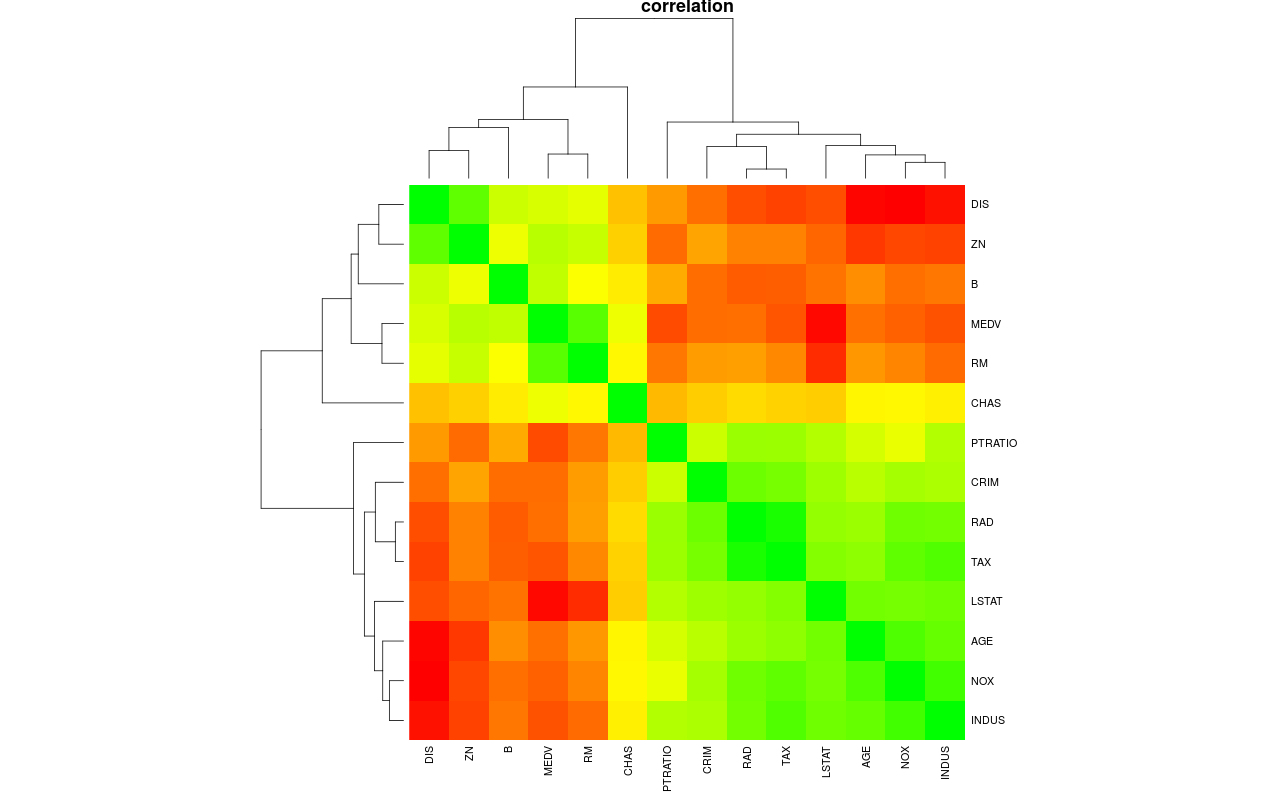
\includegraphics[scale=0.49]{correlation.png}
\caption{Show the correlation}
\end{figure}
\begin{landscape}
\begin{figure}[H]
	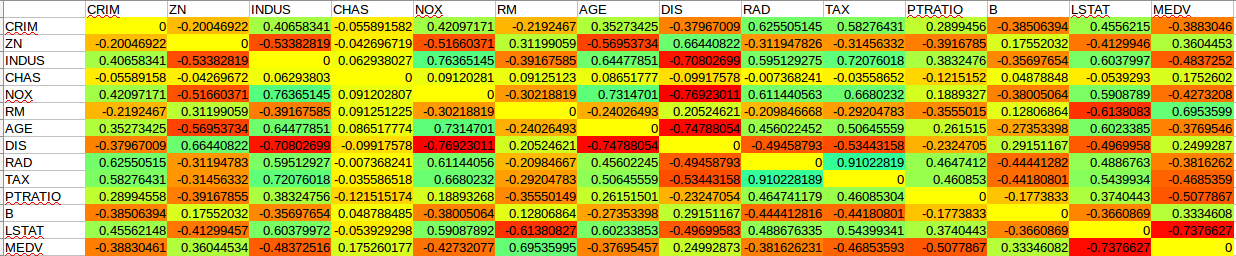
\includegraphics[scale=0.58]{heatmap2.png}
	\caption{Better look at heat map}
\end{figure}
The maximum correlation is between \(RAD,TAX\).\\
\textbf{Note: }even before executing the code, the paper we read previously mentioned implicitly that most correlated feature with the result would have the most effect.
 Let's go for the code :
 \begin{lstlisting}[language=R]
 tt<-as.data.frame(summary(lm(data = houses,MEDV~.))$coefficients)
 tt<-tt[order(-tt$Estimate),]
 tt[c(1,2),]
 \end{lstlisting} 
 The main idea for the code is just to calculate the module, get the coefficient and order them by estimation then print the first two rows (usually Intercept take the highest after it our goal row). In the following table I'll show the requested information:\\
 \begin{tabular}{|c|c|c|c|}
 	\hline
 	Class&Most effect&Most correlated&RMSD\\ \hline
 	MED&RM&RM&0.7406\\ \hline
 	CRIM&RAD&RAD&0.454\\ \hline
 	ZN&DIS&DIS&0.5749\\ \hline
 	INDUS&NOX&NOX&0.7495\\ \hline
 	CHAS&NOX&MEDV&0.08694\\ \hline
 	NOX&CHAS&INDUS&0.782\\ \hline
 	RM&MEDV&MEDV&0.5576\\ \hline
 	AGE&NOX&NOX&0.6775\\ \hline
 	DIS&CHAS&ZN&0.7725\\ \hline
 	RAD&NOX&TAX&0.8719\\ \hline
 	TAX&NOX&RAD&0.8914\\ \hline
 	PTRATIO&RAD&RAD&0.4982\\ \hline
 	B&CHAS&MEDV&0.2761\\ \hline
 	LSTAT&RAD&INDUS&0.7208\\ \hline
 \end{tabular}
\end{landscape}
From the previous table I would say B is the easer one to predict because it has the minimum RSMD.But to be honest I don't think we can say something easy or someting hard, it's just a matter of how much the features are independent from each other , and correlated from the class we are trying tp predict.
The code used for the previous table :
\begin{lstlisting}[language=R]
tt<-as.data.frame(summary(lm(data = houses,MEDV~.))$coefficients)
tt<-tt[order(-tt$Estimate),]
tt[c(1,2),]
tt<-as.data.frame(summary(lm(data = houses,CRIM~.))$coefficients)
tt<-tt[order(-tt$Estimate),]
tt[c(1,2),]
tt<-as.data.frame(summary(lm(data = houses,ZN~.))$coefficients)
tt<-tt[order(-tt$Estimate),]
tt[c(1,2),]
tt<-as.data.frame(summary(lm(data = houses,INDUS~.))$coefficients)
tt<-tt[order(-tt$Estimate),]
tt[c(1,2),]
tt<-as.data.frame(summary(lm(data = houses,CHAS~.))$coefficients)
tt<-tt[order(-tt$Estimate),]
tt[c(1,2),]
tt<-as.data.frame(summary(lm(data = houses,NOX~.))$coefficients)
tt<-tt[order(-tt$Estimate),]
tt[c(1,2),]
tt<-as.data.frame(summary(lm(data = houses,RM~.))$coefficients)
tt<-tt[order(-tt$Estimate),]
tt[c(1,2),]
tt<-as.data.frame(summary(lm(data = houses,AGE~.))$coefficients)
tt<-tt[order(-tt$Estimate),]
tt[c(1,2),]
tt<-as.data.frame(summary(lm(data = houses,DIS~.))$coefficients)
tt<-tt[order(-tt$Estimate),]
tt[c(1,2),]
tt<-as.data.frame(summary(lm(data = houses,RAD~.))$coefficients)
tt<-tt[order(-tt$Estimate),]
tt[c(1,2),]
tt<-as.data.frame(summary(lm(data = houses,TAX~.))$coefficients)
tt<-tt[order(-tt$Estimate),]
tt[c(1,2),]
tt<-as.data.frame(summary(lm(data = houses,PTRATIO~.))$coefficients)
tt<-tt[order(-tt$Estimate),]
tt[c(1,2),]
tt<-as.data.frame(summary(lm(data = houses,B~.))$coefficients)
tt<-tt[order(-tt$Estimate),]
tt[c(1,2),]
tt<-as.data.frame(summary(lm(data = houses,LSTAT~.))$coefficients)
tt<-tt[order(-tt$Estimate),]
tt[c(1,2),]
\end{lstlisting}
\section*{Sixth Question}
For this task firstly I updated the function to calculated FP,FN.\\ After that I implemented function to find the index of  minimum \(FP*15+FN*20\)
\begin{lstlisting}[language=Python]
def GetFPFN(k,dataset):
FP=0
FN=0
for i in range (3000):
#Predicted True
if i<k:
#but it's false
FP+= not original[dataset[i]]
#predicted false
else:
#but it's positive
FN+= original[dataset[i]]
#(TP,FP,TN,FN)
#(F11,F01,F10,F00)
#return (TP,TotalPositive-TP,TN,TotalNegative-TN)
#return (float (TP)/float(TotalPositive),float(k-TP)/float(TotalNegative))
return (FP,FN)

roc1cm=[]
roc2cm=[]
roc3cm=[]
roc4cm=[]
rocperfectcm=[]
print 'processing roc1'
for i in range (3000):
roc1cm.append(GetFPFN(i,roc1))
print 'processing roc2'
for i in range (3000):
roc2cm.append(GetFPFN(i,roc2))
print 'processing roc3'
for i in range (3000):
roc3cm.append(GetFPFN(i,roc3))
print 'processing roc4'
for i in range (3000):
roc4cm.append(GetFPFN(i,roc4))
print 'processing rocperfect'
for i in range (3000):
rocperfectcm.append(GetFPFN(i,rocperfect))
print 'Finished'
def FindKminimum(dataset):
k=0
lst=[]
for i in range (3000):
lst.append({'x':i,'y':dataset[i][0]*15+20*dataset[i][1]})

lst.sort(key=lambda x: x['y'], reverse=False)
return lst[0]['x']
\end{lstlisting}
After that  I used the following code to find the minimum points :
\begin{lstlisting}[language=Python]
roc1best = FindKminimum(roc1cm)
roc2best = FindKminimum(roc2cm)
roc3best = FindKminimum(roc3cm)
roc4best = FindKminimum(roc4cm)
rocperfectbest= FindKminimum(rocperfectcm)
print 'Best Points roc1:{}, roc2:{}, roc3:{}, roc4:{}, rocperfect:{}'.format(roc1cm[roc1best],roc2cm[roc2best],roc3cm[roc3best],roc4cm[roc4best], rocperfectcm[rocperfectbest])
\end{lstlisting}
Which give : 
Best Points roc1:(1058, 94), roc2:(1045, 171), roc3:(661, 376), roc4:(842, 61), rocperfect:(0, 0)\\
The following code is to find which one provide the least cost:
\begin{lstlisting}[language=Python]
def PrintTotalCost(row):
return row[0]*15+row[1]*20

print 'Best Points roc1:{}, roc2:{}, roc3:{}, roc4:{}, rocperfect:{}'.format(PrintTotalCost(roc1cm[roc1best]),
PrintTotalCost(roc2cm[roc2best]),
PrintTotalCost(roc3cm[roc3best]),
PrintTotalCost(roc4cm[roc4best]),
PrintTotalCost(rocperfectcm[rocperfectbest]))
\end{lstlisting}
The previous code print :
The cost :\( roc1:17750, roc2:19095, roc3:17435, roc4:13850, rocperfect:0\) \\ No wonder rocperfect perform the best it's the actual data reordered.But between the four models roc4 give the least cost.\\
\textbf{Note:} All Code , Tex,.ipython,.pdf,.R exist on \href{https://github.com/aqeel13932/DM/tree/master/HW09}{github}
\begin{center}
\textbf{E.O.F}
\end{center}
\begin{thebibliography}{9}
	\bibitem{1}
	\href{https://en.wikipedia.org/wiki/Receiver_operating_characteristic}{receiver operating Characteristics }
\end{thebibliography}
\end{document}
